\chapter{Part 1: Synchronization of Extreme Events}
\label{c:event_sync}
During the primary monsoon season, floodings and landslides caused by extreme rainfall can lead to massive societal and environmental damage. As we have already seen, it is crucial to be able to analyze, detect and potentially predict such extreme rainfall events, especially as their proportion tends to further increase with global warming \citep{Stolbova.2015}.

One recently proposed way for such analysis is the computation of climate networks, followed by an analysis of the resulting networks using well-known network centrality measures \citep{Stolbova.2015}. The approach taken in \citet{Stolbova.2015} has its foundations on the work of \citet{QuianQuiroga.2002}, which is why we first go over their approach to event synchronization (\cref{sst:event_synchronization}). We then summarize the principles of climate networks as applied by \citet{Stolbova.2015} in \cref{sst:climate_networks}, after which we go on to explain the network measures that will be applied to the obtained climate networks (\cref{sst:network_measures}). Before we go into any of this related work, \cref{st:trmm_dataset} first introduces the TRMM dataset that we will use in this chapter.

After going over the foundational related work, \cref{st:event_sync_implementation} provides an overview of our own approach to the creation of climate networks. Following up in \cref{st:event_sync_results}, we analyze and visualize the computed climate networks using centrality measures and try to interpret the results in contrast to the known factors of monsoon behavior. We further compare our results to the ones obtained in \citet{Stolbova.2015} and assess any apparent differences. Concluding this chapter in \cref{st:event_sync_conclusion}, we elaborate the usefulness of our results and how they could be improved upon.


\section{The TRMM Dataset}
\label{st:trmm_dataset}
The TRMM dataset is a precipitation research effort by NASA and JAXA. It is based on the TRMM observatory, a satellite that was launched into space on the 27th of November, 1997. The products based on TRMM range from the raw output of the multitude of sensors on the satellite to the highly aggregated and gridded rainfall estimates we will be using in this work \citep{GoddardEarthScienceDataInformationandServicesCenter.2016}.

More specifically, the TRMM product that we will be using is a 3-hourly estimate of surface rainfall aggregated from the satellite sensors in combination with surface gauge values and imagery from other satellites. This product is referred to as 3B42 or TMPA and is also available in a daily variation, where the eight 3-hourly measurements (i.e., 00:00, 03:00, 06:00 and so on) have been summed up to provide a single daily rainfall estimate. We use this daily TMPA product during the remainder of this work and, for simplicity, generally refer to it as TRMM.

TMPA is available for the area between 50\degree N. and 50\degree S. We subset this area to cover the entire Indian subcontinent (4.125-40.625\degree N, 61.125-97.625\degree E). These border coordinates are a small superset of the ones used in \citet{Stolbova.2015}: the grid has been extended such that it can be cleanly aggregated from a {0.25\degree} spatial resolution to the {0.75\degree} resolution of the ERA-Interim dataset we use in \cref{c:part2}. The gridded area we extracted from the TRMM dataset is visualized in \cref{fig:trmm_grid}.

\begin{figure}[h]
  \centering
  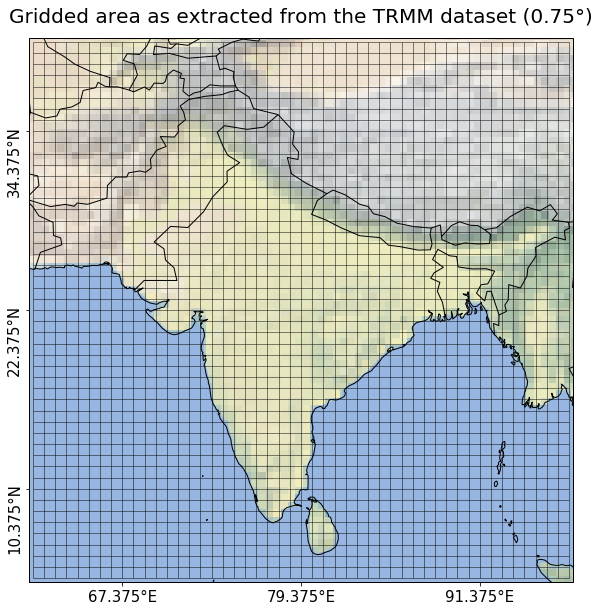
\includegraphics[width=0.5\linewidth]{./99_appendix/img/area_overview_grid}
  \caption{Overview of the Indian subcontinent as extracted from the TRMM dataset (4.125-40.625\degree N, 61.125-97.625\degree E). The TRMM dataset has been aggregated to match the {0.75\degree} resolution of the ERA-Interim dataset.}
  \label{fig:trmm_grid}
\end{figure}

The TRMM dataset is unique in that it offers very high-resolution precipitation estimates since January 1998. It can prove useful for research based on the distribution, frequency, and intensity of rainfall, i.e., for calculating extreme rainfall events \citep{Stolbova.2015}. However, it has to be taken into consideration that the TRMM products are based on complex algorithms and have been derived from different sensors and sources \citep{Huffman.2017b}.

After the TRMM satellite's fuel went low in 2014, it was decommissioned in April 2015 and re-entered earth's atmosphere in June 2015. The TMPA product is still being produced until 2018, albeit without the sensors of the TRMM observatory and with less accuracy \citep{Huffman.2017}. Built on the success of the TRMM mission, NASA and JAXA have already launched its successor Global Precipitation Measurement (GPM) in 2014 \citep{GoddardEarthScienceDataInformationandServicesCenter.2011}. However, as its data is only available starting from 2014, GPM is currently unsuitable for long-term precipitation research. TRMM or an alternative dataset are currently still needed but the updated algorithm developed for GPM will soon be applied to the existing TRMM data. The availability of reprocessed data back to 1998 can thus be expected in 2018 \citep{Huffman.2016}.

\section{Related Work}
The concept of event synchronization applied in \citet{Stolbova.2015} was first proposed in \citet{QuianQuiroga.2002}, where they sought to develop a simple algorithm that could be applied to any two time series of events, resulting in a measure that defines the synchronization of said time series. Synchronization measures are generally related to standard measures like cross correlation but can convey more complex relationships due to their non-linearity \citep{QuianQuiroga.2002}.

While the work of \citet{QuianQuiroga.2002} focuses on the analysis of electroencephalogram (EEG)\footnote{A way of measuring brain activity.} time series, their event synchronization approach is explicitly applicable to other domains. The works of \citet{Malik.2010} and \citet{Stolbova.2015} both expand upon simple event synchronization. However, they do so in different ways: \citet{Malik.2010} apply hierarchical clustering algorithms to identify different regions and their respective characteristics regarding the occurrence of extreme rainfall events. \citet{Stolbova.2015} builds ``climate networks'' and analyzes them with established network measures. For the purposes of our work, we will focus on the latter approach, using the work of \citet{Stolbova.2015} as a foundation for this chapter.

\subsection{Event synchronization}
\label{sst:event_synchronization}
The basic principle of the event synchronization measure as found in \citet{QuianQuiroga.2002} is setup as follows: given the two time series $i$ and $j$ and their respective events $l$ and $m$ occuring at times $t^i_l$ and $t_j^y$, we measure the synchronicity for all possible pairs of events between both series. We classify events as synchronous if they occur closely simultaneous, i.e., within a certain range from each other. This allowed range of occurrence is called \textit{time lag} and is calculated by taking the minimum interevent distance $\tau^{ij}_{lm}$ like so\footnote{If event rates were fixed, a global time lag $\tau$ could be defined, greatly simplifying calculations.}:

\begin{equation}
\tau^{ij}_{lm} = 0.5 * min\left\{t^i_{l+1} - t^i_l, t^i_l - t^i_{l-1}, t^j_{m+1} - t^j_{m}, t^j_{m} - t^j_{m-1}\right\}
\end{equation}

The synchronicity $J_{ij}$ of any two events $t_i^x$ and $t_j^y$ is then calculated as follows:

\begin{equation}
  J_{ij} =
  \begin{cases}
    1, & \text{if } 0<t^x_i-t^y_j\leq\tau_{ij}, \\
    0.5, & \text{if } t^x_i=t^y_j, \\
    0, & \text{else.}
  \end{cases}
\end{equation}

Applying this to the full time series $i$ and $j$, the number of synchronous events where an event in $i$ leads an event in $j$ is defined like:

\begin{equation}
  c(i \mid j) = \sum\limits^{s_i}_{l=1} \sum\limits^{s_j}_{m=1} J_{ij}
\end{equation}

The same formula applies to the reversed situation, i.e. $c(j \mid i)$.

\pagebreak
Combining the results of $c(i\mid j)$ and $c(j \mid i)$ and normalizing them by the total numbers of events $s_i$ and $s_j$, the \textit{strength of synchronization} is defined as

\begin{equation} \label{eq:sync_strength}
  Q_{ij} = \frac{c(i \mid j) + c(j \mid i)}{\sqrt{(s_i - 2)(s_j - 2)}}
\end{equation}

where $Q_{ij} = 1$ means that the time series are completely synchronized, i.e., that each event in $i$ is either synchronously lead or followed by an event in $j$.

\subsection{Climate networks}
\label{sst:climate_networks}
Looking at the TRMM dataset as shown in \cref{fig:trmm_grid}, each cell of its coordinate grid represents a separate precipitation time series. As the analysis of each monsoon season is performed seperately, one such coordinate grid per season needs to be extracted\footnote{The time series are then simply the respective months of each year, concatenated into a single series. For example: March 1998, April 1998, May 1998, March 1999, April 1999, and so on.}.

The time series in the resulting grids are not event based and thus cannot be directly used to calculate synchronization. They can, however, easily be transformed into event series by extracting only the days where extreme rainfall occurred. As per \citet{Stolbova.2015}, such days are defined as days with rainfall that exceeds the 90th percentile for the respective location.

The resulting series of extreme events can be used to calculate the synchronicity of different locations (grid cells) in the TRMM dataset, closely following the approach we have already introduced in \cref{sst:event_synchronization}. Computing the synchronicity for all possible permutations of two such locations then results in a synchronization matrix as can be seen in \cref{fig:synchronization_matrix}.

\begin{figure}[h]
  \centering
  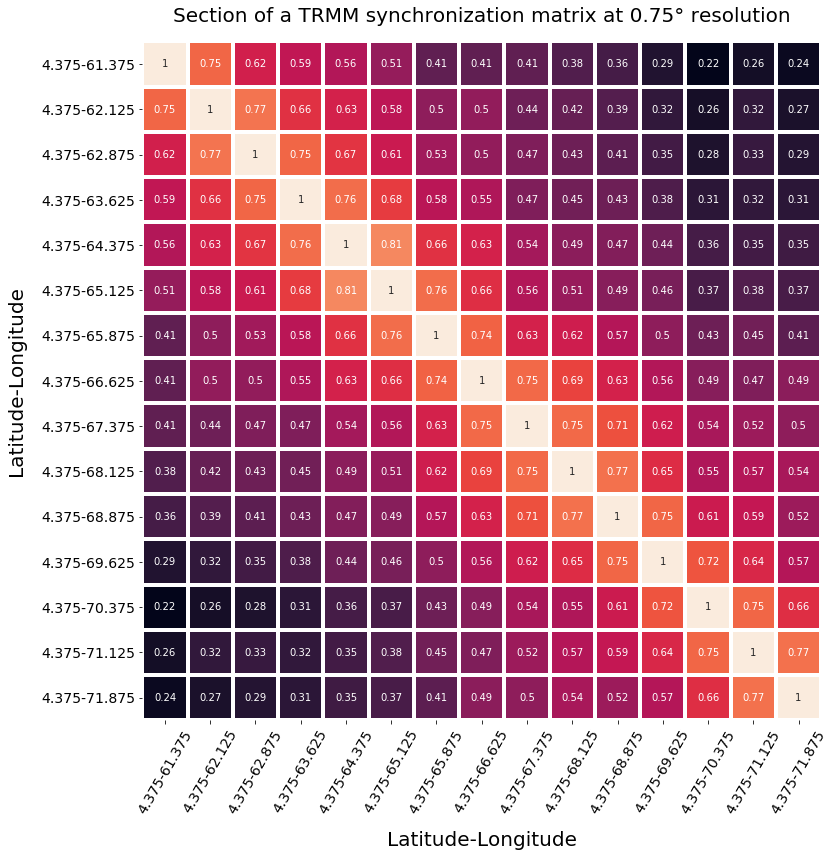
\includegraphics[width=0.5\textwidth]{./99_appendix/img/trmm_sync_example}
  \caption{Exemplary synchronization matrix for TRMM at a {0.75\degree} resolution. We only show the top left 15x15 section of our actual matrix, as its full dimensions are 2401x2401 for a {0.75\degree} resolution.}
  \label{fig:synchronization_matrix}
\end{figure}

Applying a numerical threshold to this synchronization matrix results in a matrix that contains only the most significantly synchronous values. Everything else is set to zero, including the diagonal of the matrix, as this would result in loops in the graph later on. Additionally, all elements above the threshold are set to one, yielding the adjacency matrix for an undirected, unweighted network (\cref{fig:adjacency_matrix}). \citet{Stolbova.2015} uses the 95th percentile for the threshold applied, as this removes all but the most statistically significant values.

\begin{figure}[h]
  \centering
  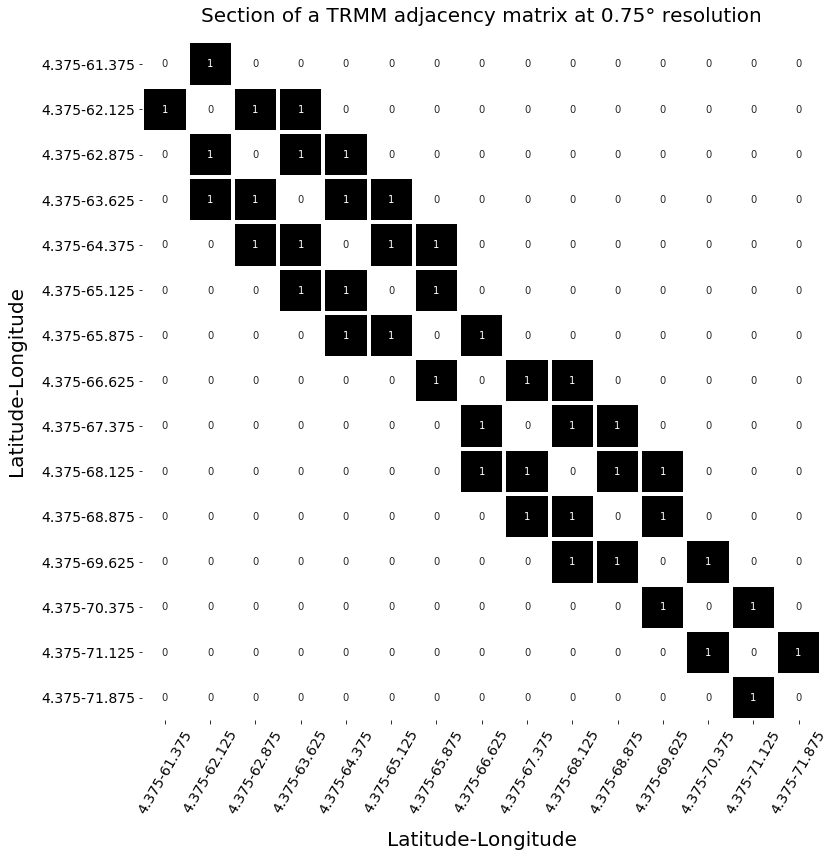
\includegraphics[width=0.5\textwidth]{./99_appendix/img/trmm_adjacency_example}
  \caption{Exemplary adjacency matrix for TRMM at a {0.75\degree} resolution. We only show the top left 15x15 section of our actual matrix, as its full dimensions are 2401x2401 for a {0.75\degree} resolution.}
  \label{fig:adjacency_matrix}
\end{figure}

Based on the adjacency matrix, a network can then be computed and analyzed. However, before we detail our implementation of it, the next section briefly describes the measures that we will be using for said network analysis.

\subsection{Network centrality}
\label{sst:network_measures}
Constructing climate networks from an adjacency matrix as seen in \cref{sst:climate_networks} enables the analysis of their structural features using various network-based measures. We now briefly introduce these measures, before we go on to apply them in the next section.

The climate networks in \citet{Stolbova.2015} are analyzed using the \textit{degree} and \textit{betweenness} of nodes as well as using the \textit{average/maximal geographical link length} between them. We also base our analysis on the \textit{degree} and \textit{betweenness} measures but replace the link length calculations with the \textit{PageRank} algorithm, which should also show interesting patterns in our opinion.

\subsubsection{Degree}
The \textit{degree} of a node in a network is quite simply defined as the number of links that are connected to this node. The same holds for vertices in graphs and their connected edges.

\subsubsection{Betweenness}
Calculating the \textit{betweenness} or \textit{betweenness centrality} of a node is a more involved effort. A node has a high betweenness if a large portion of shortest paths in the network pass through the respective node. If the resulting betweenness is to be an exact measure, this can basically necessitate the calculation of all shortest paths in the network, which gets increasingly complex with the size of the network. There are, however, algorithms that achieve both accuracy and speed when calculating betweenness, one of the most popular being the approach proposed by \citet{Brandes.2001}. This algorithm is also used by the Python library \textit{networkx}, which we will be using for our calculations.

\subsubsection{PageRank}
The final measure that we will apply to climate networks, the \textit{PageRank} algorithm, was originally developed and published by the founders of Google (amongst others), Larry Page and Sergey Brin, during their studies at Stanford University \citep{Page.1999}. Originally developed as a way to rank indexed websites by their importance, the algorithm has since been applied to a variety of other problem domains (e.g., social network analysis, neuroscience, and many others). The PageRank algorithm seeks to calculate the importance of a node in a network by taking into account its incoming and outgoing links as well as the PageRank and number of outgoing links of the thereby connected nodes (which is intuitively shown in \cref{fig:simplified_pagerank}).

\begin{figure}[h]
  \centering
  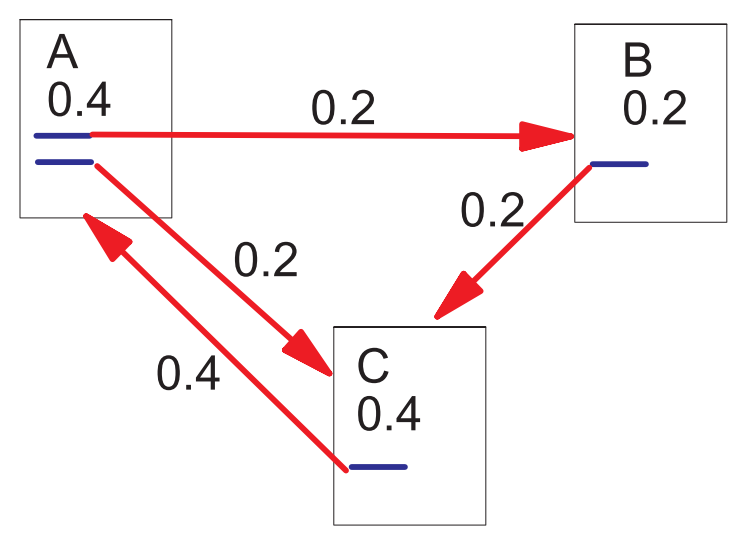
\includegraphics[width=0.4\textwidth]{./99_appendix/img/simplified_pagerank}
  \caption{The simplified PageRank algorithm as presented in \citet{Page.1999}.}
  \label{fig:simplified_pagerank}
\end{figure}

As intuitively described by \citet{Page.1999}, PageRank can be thought to model the behavior of a ``random surfer'' that simply continues clicking links on the current page, traversing the network in a random fashion. The PageRank of a particular page then represents the probability that such random surfers end up accessing the respective page. However, to prevent any random surfer from getting stuck in loops (i.e., pages that link between each other), the simplified PageRank algorithm is further extended by a teleportation capability: a random surfer will jump to a random page with probability $\alpha$, while following a link to another page with probability $1-\alpha$.

\section{Implementation}
\label{st:event_sync_implementation}
Our implementation of the event synchronization and climate network computations is strongly based on the concepts and measures as described in \cref{sst:event_synchronization} and \cref{sst:climate_networks}. As our algorithmic implementation is most certainly different than the one used in the original work \citep{Stolbova.2015}, we detail our approach in this section.

\subsection{Calculating event synchronization}
\label{sst:event_sync_calculation}
Before we are able to calculate the synchronicity for any two locations, the precipitation time series need to be transformed into series of events. Assume that we have extracted pre-monsoon precipitation time series as shown in \cref{tab:example_rainfall_ts} from the TRMM dataset and want to convert these into extreme event series.

\begin{table}[h]
  \centering
  \begin{tabular}{ cc|ccccccc }
    \toprule
    \textbf{Latitude} & \textbf{Longitude} & \textbf{01.03.98} & \textbf{...} & \textbf{29.05.98} & \textbf{30.05.98} & \textbf{31.05.98} & \textbf{01.03.99} & ...\\
    \midrule
    13.375 & 67.375 & 0.0  & ... & 0.12 & 2.31  & 2.85  & 0.00 & ... \\
    16.375 & 91.375 & 0.0  & ... & 0.09 & 34.80 & 49.49 & 0.00 & ... \\
    34.375 & 67.375 & 0.52 & ... & 0.00 & 0.00  & 0.00  & 0.00 & ... \\
    34.375 & 88.375 & 0.86 & ... & 2.01 & 51.85 & 68.72 & 0.29 & ... \\
    \bottomrule
  \end{tabular}
  \caption{Precipitation time series during pre-monsoon at 4 exemplary locations (TRMM, 0.75\degree).}
  \label{tab:example_rainfall_ts}
\end{table}

We then calculate the 90th percentile for each row and apply the result as a threshold to the respective row. This yields event series where each value represents the date of an extreme event. If applied to the time series in \cref{tab:example_rainfall_ts}, this results in event series as shown in \cref{tab:example_rainfall_events} .

\begin{table}[h]
  \centering
  \begin{tabular}{ cc|ccccccc }
    \toprule
    \textbf{Latitude} & \textbf{Longitude} & \textbf{1} & \textbf{2} & \textbf{3} & \textbf{4} & \textbf{5} & \textbf{6} & \textbf{...} \\
    \midrule
    13.375 & 67.375 & 07.04.98 & 31.05.98 & 08.05.99 & 12.05.99 & 13.05.99 & 15.05.99 & ... \\
    16.375 & 91.375 & 17.05.98 & 18.05.98 & 19.05.98 & 30.04.99 & 01.05.99 & 05.05.99 & ... \\
    34.375 & 67.375 & 03.03.98 & 29.03.98 & 02.04.98 & 03.04.98 & 09.04.98 & 22.04.98 & ... \\
    34.375 & 88.375 & 18.03.98 & 30.03.98 & 31.03.98 & 01.04.98 & 05.04.98 & 19.04.98 & ... \\
    \bottomrule
  \end{tabular}
  \caption{Events in the pre-monsoon extreme event series at 4 exemplary locations (TRMM, 0.75\degree).}
  \label{tab:example_rainfall_events}
\end{table}

Going forward, we use \textit{epoch timestamps} to represent dates instead of the full representation shown in the examples of this section, as they are much easier to process using mathematical formulas (but less intuitive to visualize). Epoch timestamps measure the number of seconds (without leap seconds) that have elapsed since the 01.01.1970 at 00:00 UTC. For example, \textit{01.03.1998 00:00} would be represented as \textit{888710400}. An exemplary event series based on epoch timestamps is presented in \cref{tab:example_rainfall_events_unix}. Such timestamps or similar numerical representations are internally used in many applications and algorithms, as calculating differences between dates or shifting a date is as simple as performing mathematical addition or subtraction operations.

\begin{table}[h]
  \centering
  \begin{tabular}{ cccccccc }
    \toprule
    \textbf{Event} & \textbf{1} & \textbf{2} & \textbf{3} & \textbf{4} & \textbf{5} & \textbf{6} & \textbf{...} \\
    \midrule
    \textbf{Date} & 07.04.98 & 31.05.98 & 08.05.99 & 12.05.99 & 13.05.99 & 15.05.99 & ... \\
    \textbf{Epoch} & 891907200 & 896572800 & 926121600 & 926467200 & 926553600 & 926726400 & ... \\
    \bottomrule
  \end{tabular}
  \caption{Exemplary series of events represented with epoch timestamps (TRMM, 0.75\degree).}
  \label{tab:example_rainfall_events_unix}
\end{table}

\subsubsection{Synchronization of two locations}
Having explained the necessary setup of the event synchronization algorithm, we now focus on more concrete aspects of our implementation. To calculate the synchronization between any two locations (i.e., \textit{location1} and \textit{location2}), we need to process both time series and compare each event in \textit{location1} to the appropriate events in \textit{location2}, taking the immediate neighbors of both locations into account. We found that this naturally fits the description of a \textit{sliding window} approach: a sliding window of size three over the event series of a location always encompasses a current event, its predecessor and its successor and thus everything we need for the time lag calculation. Application of a sliding window to \textit{location1} and nesting another such window for \textit{location2} then leads us to the naive implementation shown in \cref{lst:event_synchronization}\footnote{Notice that to allow sliding windows to go from the very first to the very last event, additional padding needs to be applied on either side. We pad with the timestamps 0 and 9999999999, preventing any influence on time lags.}.

\begin{listing}[h]
  \begin{minted}[mathescape,
    linenos,
    numbersep=5pt,
    gobble=4,
    frame=lines,
    framesep=2mm]{python}

    def calculate_synchronization(location1, location2):

        # initialize the number of synchronous events for the two locations
        num_sync_events = 0

        # iterate over all timesteps in location1 using a sliding window
        for i_prev, i_current, i_next in sliding_window(location1, 3):

            # iterate over all timesteps in location2 using a sliding window
            for j_prev, j_current, j_next in sliding_window(location2, 3):

                # calculate the time delta between the current events
                current_diff = j_current - i_current

                # check if the current events occur simultaneously
                if current_diff == 0:
                    num_sync_events += 0.5
                    continue

                # calculate the time lag based on the two sliding windows
                time_lag = 0.5 * min(
                    i_next - i_current, i_current - i_prev,
                    j_next - j_current, j_current - j_prev)

                # decide whether the events are synchronous
                if 0 < current_diff <= time_lag:
                    num_sync_events += 1.0

        return num_sync_events

  \end{minted}
  \caption{Python pseudocode for a simplified event synchronization algorithm, applicable to any two series of events represented by epoch timestamps.}
  \label{lst:event_synchronization}
\end{listing}

The event synchronization algorithm as described in \cref{lst:event_synchronization} results in the number of synchronous events between \textit{location1} and \textit{location2} where the event in \textit{location1} leads the event in \textit{location2} (i.e., $c(\text{location1} \mid \text{location2})$). The above is, however, only part of the full synchronization calculation, as we also need the number of synchronous events where \textit{location1} leads \textit{location2}, i.e., we need to evaluate $c(\text{location2} \mid \text{location1})$. This is the reason that simultaneous events only count as "half synchronous": they are counted in both these calculations and, in total, then result in one synchronous event.

Calculating the strength of synchronization boils down to a simple application of \cref{eq:sync_strength} from Page \pageref{eq:sync_strength} and is further presented in \cref{lst:sync_strength}. Notice that, in addition to the synchronization coefficient, we return both numbers of synchronous events (i.e., $c(i \mid j)$ and $c(j \mid i)$). This is used to build a directed network later on.

\begin{listing}[h]
  \begin{minted}[mathescape,
    linenos,
    numbersep=5pt,
    gobble=4,
    frame=lines,
    framesep=2mm]{python}

    def calculate_sync_strength(loc1_events, loc2_events):

        # calculate synchronized events between loc1 and loc2 (and reverse)
        loc1_sync = calculate_synchronization(loc1_events, loc2_events)
        loc2_sync = calculate_synchronization(loc2_events, loc1_events)

        # calculate the strength of synchronization
        sync_strength = (loc1_sync + loc2_sync) / \
            math.sqrt((len(loc1_events) - 2) * (len(loc2_events) - 2))

        # return the strength of synchronization
        # and the total and separate numbers of synchronous events
        return sync_strength, loc1_sync + loc2_sync, loc1_sync, loc2_sync

  \end{minted}
  \caption{Python pseudocode for the calculation of the synchronization strength between any two series of events.}
  \label{lst:sync_strength}
\end{listing}

\subsubsection{Computing the values of the synchronization matrix}
Given a matrix of extreme events as shown in excerpt in \cref{tab:example_rainfall_events} (but based on epoch timestamps), we want to calculate the synchronization coefficient and the number of synchronous events for all pairs of locations. \cref{tab:example_empty_sync} shows the state of a preliminary synchronization matrix before running any of the calculations. Locations are always perfectly synchronous to themselves, leading to a diagonal that is always filled with ones (in the case of a synchronization coefficient matrix).

\begin{table}[h]
  \centering
  \begin{tabular}{ cccccc }
    \toprule
     & \textbf{Latitude} & \textbf{13.375} & \textbf{16.375} & \textbf{34.375} & \textbf{34.375} \\
     \textbf{Latitude} & \textbf{Longitude} & \textbf{67.375} & \textbf{91.375} & \textbf{67.375} & \textbf{88.375} \\
    \midrule
    13.375 & 67.375 & 1 &   &   &   \\
    16.375 & 91.375 &   & 1 &   &   \\
    34.375 & 67.375 &   &   & 1 &   \\
    34.375 & 88.375 &   &   &   & 1 \\
    \bottomrule
  \end{tabular}
  \caption{``Empty'' synchronization matrix for 4 exemplary locations (TRMM, 0.75\degree).}
  \label{tab:example_empty_sync}
\end{table}

Next to a synchronization matrix that contains all synchronization coefficients ($Q_{ij}$), we want to generate two more matrices with the same dimensions: one matrix containing the total count of synchronous events for all pairs of locations ($c(i \mid j) + c(j \mid i)$) as well as a matrix that seperately contains the results of $c(i \mid j)$ and $c(j \mid i)$ (and is thus asymmetrical). We can generate all three of these matrices in a single pass, as $c(i \mid j)$ and $c(j \mid i)$ are intermediate results when calculating $Q_{ij}$. The procedure is shown in detail in \cref{lst:sync_matrix}.

\begin{listing}[h]
  \begin{minted}[mathescape,
    linenos,
    numbersep=5pt,
    gobble=4,
    frame=lines,
    framesep=2mm]{python}

    def calculate_sync_matrix(event_matrix):

        # calculate the sync strength for each permutation of grid cells
        for i in range(0, sync_matrix.shape[0]):

            # as the matrix is symmetrical, only calculate the upper half
            for j in range(0, i + 1):

                # calculate the synchronicity for the permutation of rows
                sync_strength, count = calculate_sync_strength(
                    event_matrix[i], event_matrix[j])

                # save results in the respective matrices
                sync_matrix[i, j] = sync_strength
                sync_matrix[j, i] = sync_strength
                count_matrix[i, j] = count
                count_matrix[j, i] = count
                directed_matrix[i, j] = i_leads
                directed_matrix[j, i] = j_leads

        return sync_matrix, count_matrix, directed_matrix

  \end{minted}
  \caption{Python pseudocode for processing an entire event matrix.}
  \label{lst:sync_matrix}
\end{listing}

\subsubsection{Improvements for the event synchronization algorithm}
The implementation as shown so far naively processes all possible combinations of events when calculating the event synchronization measure. Given two event series $i$ and $j$ as well as their respective number of events $s_i$ and $s_j$, the simple nested loop algorithm potentially calculates synchronicity up to $s_i * s_j$ times. This results in a lot of wasted computation, because the actual portion of $j$ that can be synchronous tends to be very small.

However, we can define a range of events in $j$ for which we are sure that they cannot be synchronous and entirely skip their evaluation. According to our implementation, this holds for two cases: firstly, if the event in $j$ occurs earlier than the event in $i$, it can be safely skipped, as the reversed iteration of the algorithm will deal with it. Secondly, an event in $j$ can be skipped if the event in $j$ occurs earlier than the partial time lag of the event in $i$, as the minimum of the full time lag calculation will never change. In such a case, we can additionally break the inner loop early, as further events in $j$ would only occur even later. A version of the algorithm incorporating these improvements is shown in \cref{lst:event_synchronization_improved}.

Another (obvious) improvement would be to select only the few relevant events from $j$ using advanced indexing and selection strategies, after which no more breaking or skipping in the loop would be needed. However, upon evaluation of such an approach, it became clear that this is not necessarily faster. Adequately selecting only relevant events from the series $j$ necessitates some complex indexing and selection operations, which in turn depend on the existence of an index or hash table for $j$. Creating such indices can take more than a second for a single series, making the approach especially slow for large matrices (as index creation is repeated $i$ times).

\begin{listing}[H]
  \begin{minted}[mathescape,
    linenos,
    numbersep=5pt,
    gobble=4,
    frame=lines,
    framesep=2mm]{python}

    def calculate_synchronization(location1, location2):

        # initialize the number of synchronous events for the two locations
        num_sync_events = 0

        # iterate over all timesteps in location1 using a sliding window
        for i_prev, i_current, i_next in sliding_window(location1, 3):

            # calculate the last timestamp of location2 that could be synchronous
            latest = i_current + 0.5 * min(i_current - i_prev, i_next - i_current)

            # iterate over all timesteps in location2 using a sliding window
            for j_prev, j_current, j_next in sliding_window(location2, 3):

                # calculate the time delta between the current events
                current_diff = j_current - i_current

                # if the difference is negative, continue (too early)
                # the second pass will encompass these combinations
                if current_diff < 0:
                    continue

                # check if the events occur simultaneously
                if current_diff == 0:
                    num_sync_events += 0.5
                    continue

                # break for timestamps that cannot possibly be synchronous
                # i.e. are much too late
                if j_current > latest:
                    break

                # calculate the time lag based on the two sliding windows
                time_lag = 0.5 * min(
                    i_next - i_current, i_current - i_prev,
                    j_next - j_current, j_current - j_prev)

                # decide whether the events are synchronous
                if 0 < current_diff <= time_lag:
                    num_sync_events += 1.0

        return num_sync_events

  \end{minted}
  \caption{Python pseudocode for an improved version of the event synchronization algorithm, applicable to any two series of events.}
  \label{lst:event_synchronization_improved}
\end{listing}

A further performance consideration is the fact that the event synchronization calculation $c(i \mid j)$ is in itself an ``elementary'' operation that will provide results based on only two inputs $i$ and $j$ without any side effects. As a result, the entire synchronization matrix computation is heavily parallelizable, meaning that we can split the synchronization matrix into different jobs and run these jobs on different threads (or even machines). We have already implemented an (experimental) parallelized version of the event synchronization algorithm. The parallelized algorithm will, however, need further refinement to be fully applicable.

\subsection{Building climate networks}
\label{sst:building_climate_network}
Based on \cref{sst:climate_networks}, the next step after the computation of a full event synchronization matrix is the transformation of said matrix into an adjacency matrix, allowing the creation of a network and its analysis using various methods and libraries. This transformation is a simple thresholding of the matrix using a specified percentile.

We further expand upon the work of \citet{Stolbova.2015} in two major ways: firstly, we build weighted networks in addition to the unweighted networks that have already been explored. To build a weighted network, values above the threshold are left as is, leading to links that are weighted with their corresponding synchronization measure. Contrarily, all values above the threshold are uniformly set to one when building an unweighted network. As a second addition, we build a directed network, meaning that we use an asymmetrical adjacency matrix based directly on the number of synchronous events (instead of combining both counts into a single synchronization coefficient). A directed network is  much more appropriate for an analysis using PageRank, as the results of PageRank on an undirected network are relatively similar to the degree of such a network.

The creation of a climate network based on a synchronization matrix, as well as the calculation of the degree, betweenness and PageRank for all nodes in the network, are a matter of a few lines of code as shown in \cref{lst:climate_networks}. Once the climate network computations have successfully finished, we are ready to visualize and interpret the results, which will be the major focus of the next section.

\begin{listing}[h]
  \begin{minted}[mathescape,
    linenos,
    numbersep=5pt,
    gobble=4,
    frame=lines,
    framesep=2mm]{python}

    # extract the 95th percentile from a synchronization matrix
    95th_percentile = np.nanpercentile(sync_matrix, 95)

    # set all values above and below the threshold to 0 and 1
    adjacency_matrix[adjacency_matrix > 95th_percentile] = 1
    adjacency_matrix[adjacency_matrix <= 95th_percentile] = 0

    # build a network from the resulting adjacency matrix
    network = nx.from_numpy_matrix(adjacency_matrix)

    # calculate the degree, betweenness and PageRank for all nodes
    nodes_degree = network.degree()
    nodes_betweenness = nx.betweenness_centrality(network)
    nodes_pagerank = nx.pagerank_numpy(network)

  \end{minted}
  \caption{Simplified Python pseudocode for the creation of a climate network from a synchronization matrix as well as the calculation of corresponding network measures.}
  \label{lst:climate_networks}
\end{listing}

\section{Results \& Evaluation}
\label{st:event_sync_results}
This sections presents the results of applying what we have described in \cref{st:event_sync_implementation} to the TRMM dataset, more specifically the pre-monsoon, monsoon and post-monsoon seasons as extracted from TRMM. For each season, we show the results of degree, betweenness and PageRank measures in their weighted variation\footnote{The unweighted versions can be found in \cref{apx:event_sync}. There is, however, only little difference between them.}. The presented PageRank results are based on the corresponding asymmetrical synchronization count matrices (directed networks). Knowing about the fundamental factors that influence the ISM (as introduced in \cref{c:ism_overview}), we give our thoughts about the patterns that can be seen in the results and how they could be connected to the fundamental behavior of the ISM.

\subsection{Dataset}
The results presented in this section are based on the TRMM dataset as introduced in \cref{st:trmm_dataset}. We have extracted data for the years 1998-2016, which corresponds to all years that were fully available at the time (March-December). The area included in the dataset is cropped to an extended overview over the Indian subcontinent (4.125-40.625N, 61.125-97.625E). Aggregation of the native {0.25\degree} resolution to a lower {0.75\degree} resolution yields grid borders equal to 4.375-40.375N, 61.375-97.375E (as shown in \cref{fig:trmm_grid}). The dataset was aggregated to reduce the computational effort required for event synchronization and climate network calculations. Going from {0.25\degree} to {0.75\degree} resolution effectively reduced the dimensions of the event synchronization matrices from 21609x21609 to around 2401x2401 (a reduction factor of 81x). The reduced resolution further ensures compatibility with the ERA-Interim dataset used later on.

\subsection{Pre-monsoon season (MAM)}
The results of applying our algorithms to the pre-monsoon season, namely the months of March, April and May (MAM), are shown in \cref{fig:results_mam}. We therein show the weighted network measures for a climate network thresholded by both its 95th and 90th percentile. The unweighted versions of all visualizations can be found in \cref{apx:event_sync}.

\begin{figure}[h]
  \centering
  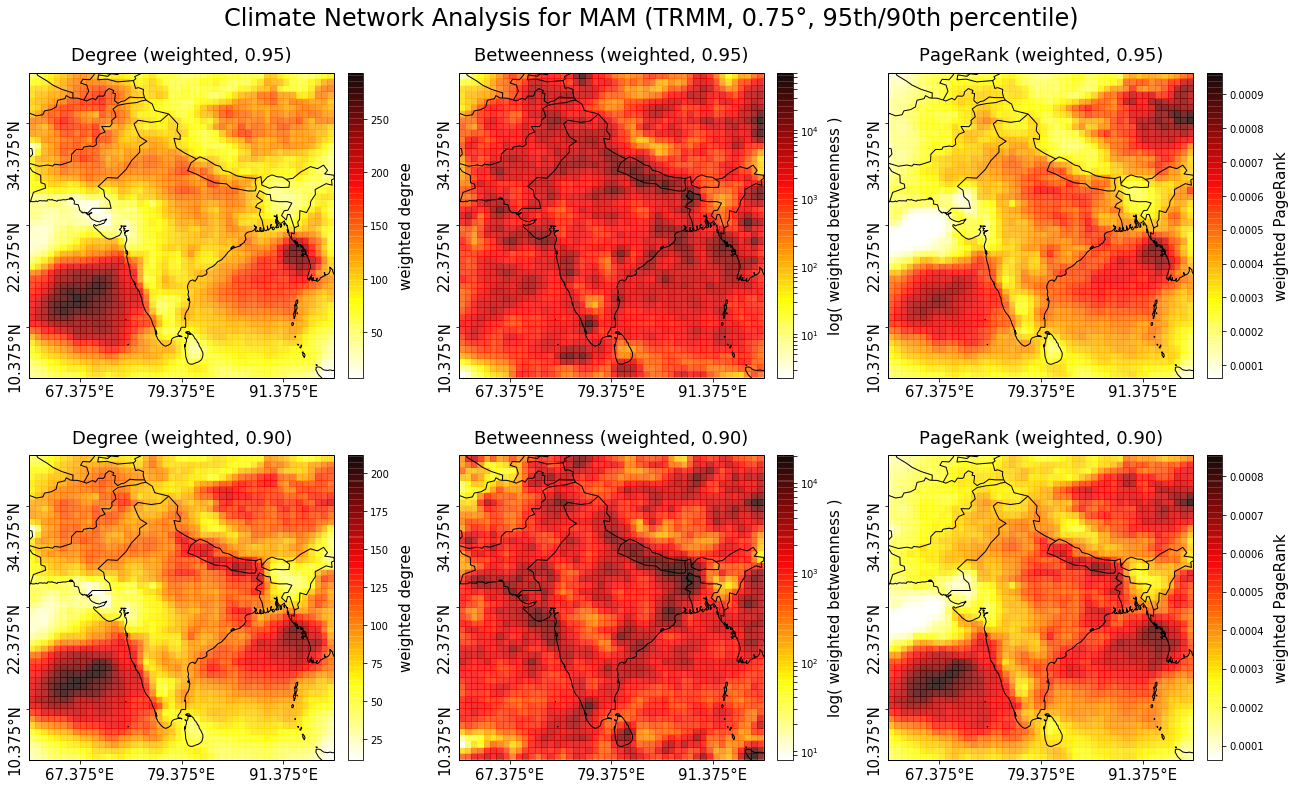
\includegraphics[width=\textwidth]{{./99_appendix/img/event_sync_0.75-0.9_MAM_both}.png}
  \caption{Weighted degree, betweenness and PageRank for the pre-monsoon season (MAM), thresholded with both the 95th and the 90th percentile. Based on the TRMM dataset at {0.75\degree} resolution.}
  \label{fig:results_mam}
\end{figure}

The degree is strongest over the Indian ocean, enframing the Indian subcontinent from both east and west. On the western side lies the Arabian Sea, over which an area of high degree extends from the far west up to the natural barrier of the Western Ghats mountain range (WG). A similar but smaller area over the Bay of Bengal to the east of the Indian subcontinent ranges from the Indian coast onto the lands of Myanmar (BoB). Further patches of significant degree can be found over the Tibetan Plateau (TP), over north-eastern India and Nepal at the brim of the Himalayas (Himalayas) and over areas of Pakistan and Afghanistan (NP, representing North-Pakistan).

Many patterns in the betweenness are much less clear and conclusive. There are, however, still spots that display significantly high betweenness, especially the area over Nepal (Himalayas). Additionally, smaller patches of high betweenness are sprinkled over the Tibetan Plateau (TP), to the north of Pakistan and over central India.

Our final measure, the PageRank algorithm, seems to follow the major patterns we have already seen in the degree. However, contrary to the degree, PageRank attributes very little importance to the region to the north-west of India. Instead, central India and especially the Tibetan Plateau are ranked to be much more important.

During the pre-monsoon or "summer" season, rainfall in southern or central India is a rare occasion, as can be seen in \cref{apx:trmm_prec}. Temperatures during these hot summer months range around 30-40\degree Celsius (\cref{apx:era_t}), even causing drought-like conditions in some years. This coincides well with our findings that the most central parts of the network are located in big clusters over the Indian ocean: as the ocean temperatures are lower than the ones on the subcontinent, wind channels moisture away from the land and onto the ocean.

However, the centrality of a location does not (necessarily) represent the amount of rainfall but the overall ``importance'' of a location in the network, which is harder to reason about. For example, a location can obtain high degree centrality simply because it is part of many large-scale events like thunderstorms that cause high or even extreme precipitation in a large area, which would certainly explain the clusters over the ocean.

Furthermore, the significant degree and high betweenness at the brim of the Himalayas could be caused by its connectedness to either one or both clusters over the Indian ocean. As an area displaying high betweenness lies on a large portion of shortest paths in the network, a connection of the cluster over the Bay of Bengal to the Himalayas certainly makes sense. This would also be supported by the general importance of the Himalaya region as a "monsoon trough" that serves as an entry point to the subcontinent for moisture from the Bay of Bengal (see \cref{c:ism_overview}).

\subsection{Monsoon season (JJAS)}
Analyzing the months of the primary monsoon season (JJAS, June-September) as shown in \cref{fig:results_jjas} yields somewhat unexpected results: degree, betweenness and PageRank all display a strong but compact pattern over Northern Pakistan (NP), especially when thresholded at the 90th percentile. Further areas of significant degree are located on the Tibetan Plateau (TP) and over the Indian Ocean around the southern tip of India (Arabian Sea/WG and BoB). High betweenness can be seen over Northern Pakistan (NP), near the Western Ghats (WG) and Kerala as well as on the other side of the southern tip of India.

\begin{figure}[h]
  \centering
  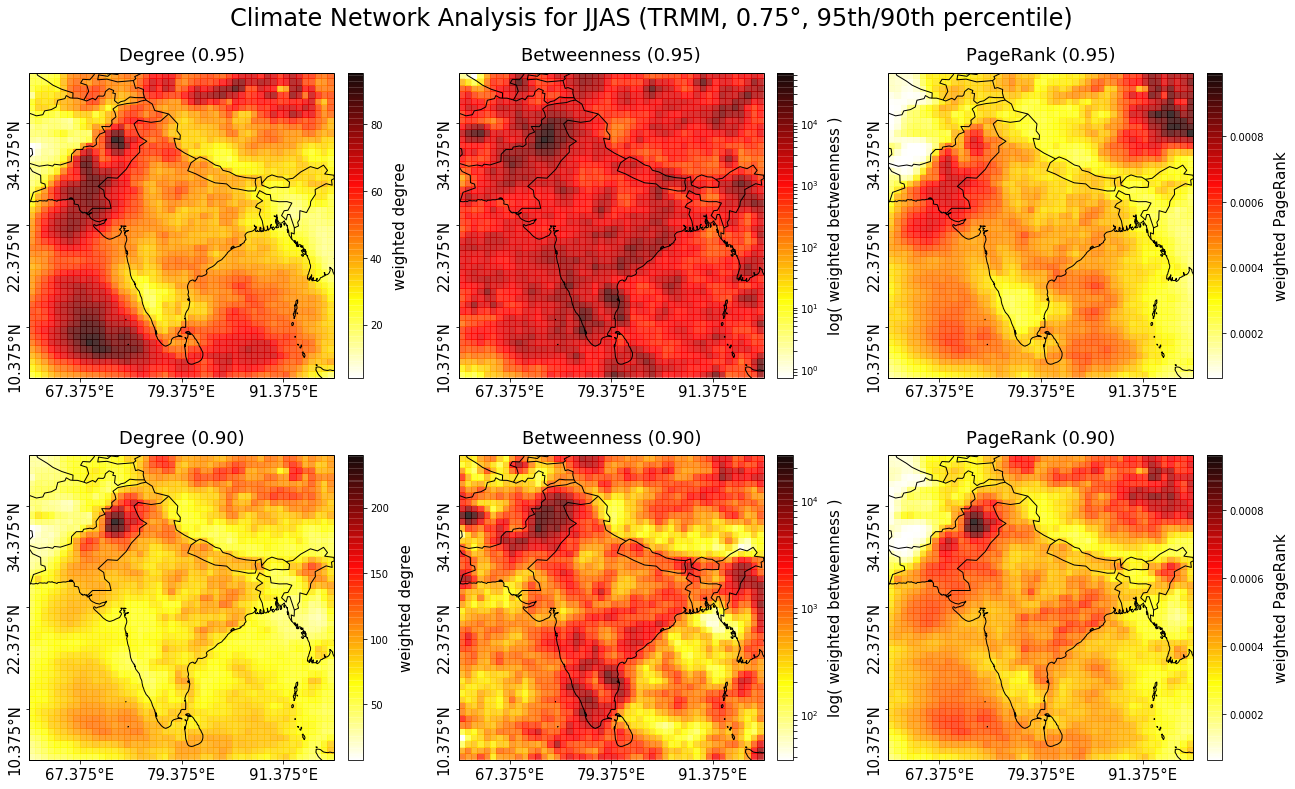
\includegraphics[width=\textwidth]{{./99_appendix/img/event_sync_0.75-0.9_JJAS_both}.png}
  \caption{Weighted degree, betweenness and PageRank for the monsoon season (JJAS), thresholded with both the 95th and the 90th percentile. Based on the TRMM dataset at {0.75\degree} resolution.}
  \label{fig:results_jjas}
\end{figure}

Having locations of high degree and high betweenness clustered over a region like Northern Pakistan suggests that even such a small region can be a great influence to many parts of the Indian subcontinent. However, it is hard to reason where the region's importance stems from. Perhaps it serves as a pivot between the Tibetan Plateau, the Arabian Sea and central India and thus is very central and part of many paths in the network.

The regions of strong betweenness flanking the Western Ghats could be explained by the important role of the Kerala region in the overall onset of the monsoon season. Kerala is typically the first region of the Indian subcontinent that is reached by monsoonal rainfalls. Thus, it can be argued that extreme events in Kerala tend to lead events on the mainland and are most probably connected to many locations in India. Furthermore, the jet coming from the Arabian Sea are split into two streams due to the heights of the Western Ghats. Continuing into the mainland, these two streams could be a cause for the patterns of high betweenness on either side of the Western Ghats.

As it already has in the pre-monsoon season, the PageRank algorithm seems to attribute great importance to the Tibetan Plateau. The Tibetan Plateau is, in fact, one of the major drivers of the ISM, as its intense heating during the summer months and the resulting winds bring high amounts of moisture onto the subcontinent. With that being said, the plateau itself doesn't receive as much rainfall as many other parts of India, as we can see in \cref{apx:trmm_prec}. The most probable reason for it being ranked as high is that it is strongly connected to the important region over North Pakistan.

\subsection{Post-monsoon season (OND)}
Contrary to the pre-monsoon season, the months of the post-monsoon season (OND, October-December) can be thought of as the Indian winter months. During these winter months, the ISM retreats completely, giving lead to the north-east monsoon towards the end of the year. The patterns as shown in \cref{fig:results_ond} seem to largely track this retreat of the ISM.

\begin{figure}[h]
  \centering
  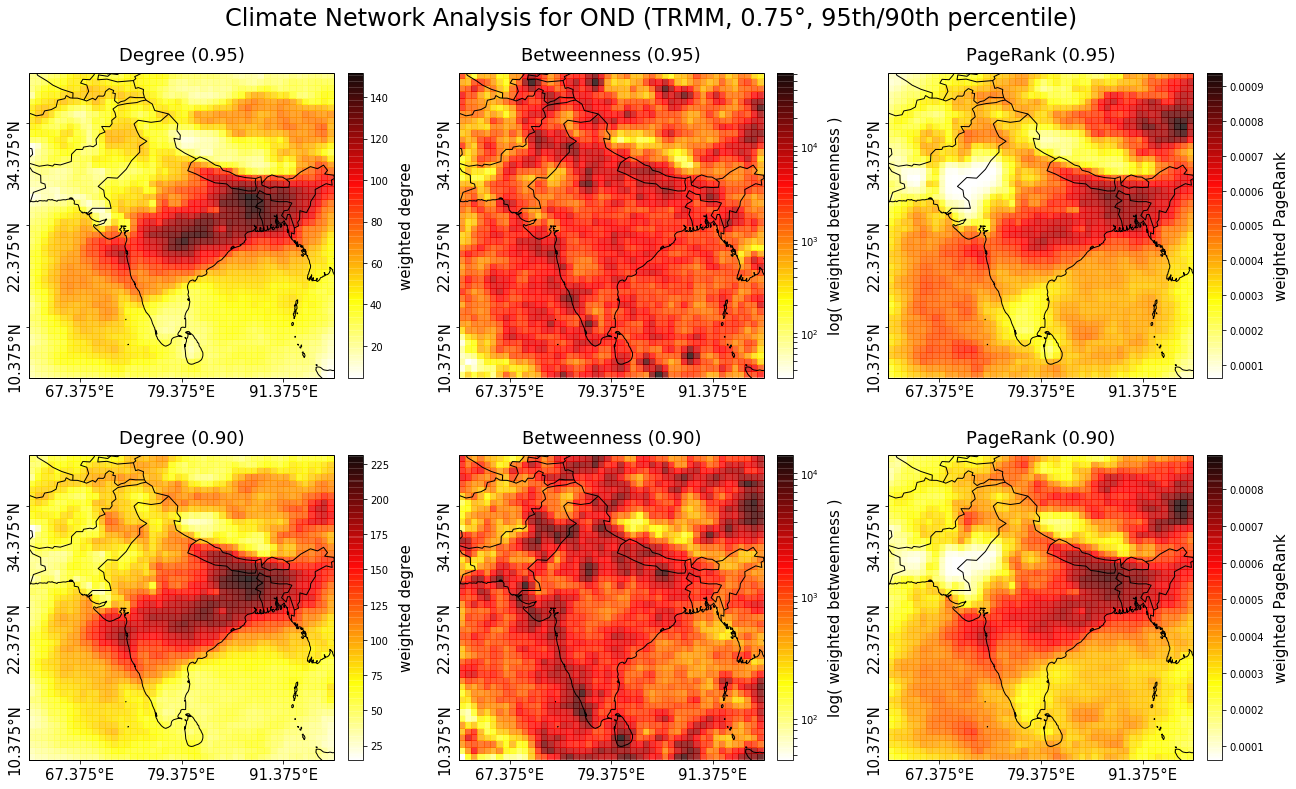
\includegraphics[width=\textwidth]{{./99_appendix/img/event_sync_0.75-0.9_OND_both}.png}
  \caption{Weighted degree, betweenness and PageRank for the post-monsoon season (OND), thresholded with both the 95th and the 90th percentile. Based on the TRMM dataset at {0.75\degree} resolution.}
  \label{fig:results_ond}
\end{figure}

More specifically, a single area of very high degree encompasses entire central and north-eastern India, starting over the Arabian Sea (WG) and ranging well into Bangladesh. The degree in this area is at its highest over Nepal close to the Himalayas. The area further extends over the Tibetan Plateau (TP), although with less strength. Similarly, areas of high betweenness are located over Nepal, at the coast of the Arabian Sea, over North Pakistan (NP) and on the Tibetan Plateau (TP). The PageRank algorithm again seems to rank the Tibetan Plateau region as more important than the other two measures.

We mainly attribute the pattern of high degree and PageRank to the retreat of the ISM as well as the following buildup-phase of the north-east monsoon. During the later parts of the year, some locations experience more rainfall than even during monsoon. As the land cools down faster than the oceans surrounding it, the temperature gradient reverses, causing winds to change direction. This can dramatically change the spatial distribution of rainfall and could thus be a reason for the difference in patterns between the monsoon and post-monsoon periods.

\subsection{Intercomparison with \citet{Stolbova.2015}}
This section shows the results as they have been presented in the referred work \citep{Stolbova.2015} and compares them to the results we have obtained from our own analysis. Next to giving an indication about the validity of our approach, this might also show new properties that have only recently developed, as we have had access to four additional years of the TRMM dataset.

\subsubsection{Differences in implementation}
The calculations and results in \citet{Stolbova.2015} are based on unweighted climate networks with event series containing only the events above the 90th percentile. Furthermore, the climate networks are thresholded at the 95th percentile, leaving only the most statistically significant edges in a network. We have calculated the degree and betweenness measures in similar ways. There are, however, certain important differences and additions in our implementation that need to be taken into account when comparing the results of both works. These differences can be categorized in the following three categories:

\paragraph{PageRank and directed networks}
As a new measure, we have calculated the PageRank of climate networks, expecting to get further insights about the importance of locations. As the PageRank algorithm works best on directed networks, we have additionally computed directed variations of each network and network measure.

\paragraph{Weighted networks}
The climate network analyses as shown so far are based on weighted climate networks, where each link between two locations is weighted with the respective synchronization coefficient. While we have found this to represent certain details differently, the overall differences are small.

\paragraph{Dataset resolution}
We have aggregated the TRMM dataset to a {0.75\degree} resolution by summarizing patches of 3x3 grid cells into one single grid cell. We have done this mainly due to performance reasons, as the full synchronization matrix for a native {0.25\degree} resolution restricted to our area has dimensions of 21609x21609, making traversal of the matrix a computationally very complex effort (compared to a 2401x2401 matrix using {0.75\degree} resolution).

\paragraph{Network thresholding}
As the much lower resolution of our TRMM input reduces the size of the networks by a large proportion, we have decided to perform an additional evaluation at the 90th percentile, trading off less significance for bigger networks.
\\ \\
\cref{apx:event_sync} contains an overview of the climate networks we have created, taking into account their differentiation into unweighted/weighted and directed/undirected networks.

\subsubsection{Differences in results}
While we have already shown the differences between the implementation of both \citet{Stolbova.2015} and our work, the network measures that finally result also exhibit some different characteristics. The visualizations as shown in \cref{fig:results_stolbova} have been extracted from \citet{Stolbova.2015} and will now be used to provide an overview about these differences in our results.

\begin{figure}[H]
  \centering
  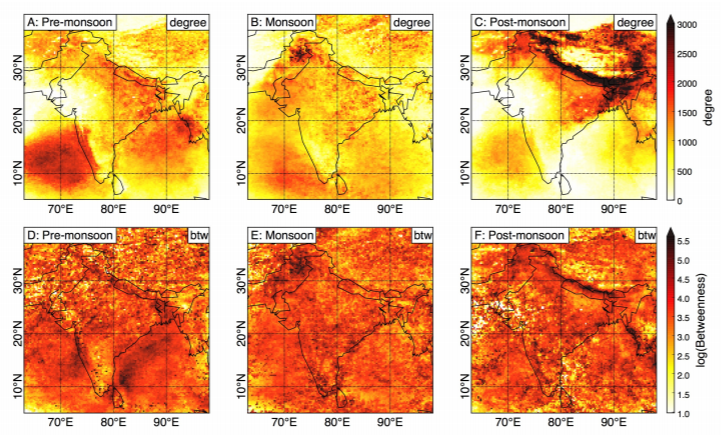
\includegraphics[width=\textwidth]{./99_appendix/img/results_stolbova.png}
  \caption{Degree and betweenness centrality as presented in \citet{Stolbova.2015}. Based on the years 1998-2012 from the TRMM dataset at {0.25\degree} resolution.}
  \label{fig:results_stolbova}
\end{figure}

The visualizations as shown in \cref{fig:results_stolbova} are obviously much more granular and detailed, as the full {0.25\degree} resolution was used for the climate network computations, while we have used a {0.75\degree} resolution. However, the general patterns seem to overlap well for the first two monsoon seasons. The main regions of interest during the pre-monsoon season are similarly located over the Arabian Sea, the Bay of Bengal, south of the Himalayas and on the Tibetan Plateau. The monsoon season shows the same strong clustering over North Pakistan and significant patterns at the southern tip of India as well as over the Arabian Sea.

Comparing the results for the post-monsoon season, we find that the discrepancies are much more significant. While the most central locations are clustered around the Himalayas in both \cref{fig:results_ond} and \cref{fig:results_stolbova}, the area of high degree extends much farther to the west in our results. Additionally, the results as shown in \cref{fig:results_stolbova} seem to be more concentrated to the Himalaya region and extend far up on the Tibetan Plateau. However, while the degree doesn't match all that well, the PageRank seems to acurately recognize the importance of the Tibetan Plateau during the post-monsoon season.

We mainly attribute the observed discrepancies to two important factors: the choice of resolution and the availability of data. We have used a lower data resolution to be able to speed up computation of the synchronization matrix and climate networks. It is obvious that a higher resolution leads to much more detailed results. Furthermore, the choice of resolution probably also has an impact on the general structure of a network, as a {0.25\degree} resolution results in a matrix that is much more sparse than it is after aggregation. An additional non-negligible factor is the availability of four additional years of TRMM data. We have been able to use the years 1998-2016 instead of 1998-2012, which corresponds to an increase of more than 25\%. The trend that causes extreme events to occur more and more often would certainly also be capable of causing significant changes in the spatial distribution of extreme events, which might further explain the differences between our results.

\section{Conclusion}
\label{st:event_sync_conclusion}
In this part of our work, we have introduced the concepts of event synchronization and climate networks and have applied them for the analysis of extreme rainfall events on the Indian subcontinent. We have applied established network measures like betweenness centrality and PageRank to climate networks, allowing us to make observations about the importance of different regions on the Indian subcontinent (with respect to extreme rainfall).

During the pre-monsoon season, the Indian Ocean and the Tibetan Plateau were identified as the most central regions in the network. We have attributed this to their importance during the reversal of the temperature gradient due to unequal solar heating and due to the fact that most rainfall during the pre-monsoon season is concentrated over the oceans, while the subcontinent remains very dry.

For the monsoon season, a region over North Pakistan was surprisingly attributed the highest levels of centrality by all measures. While this is coherent with the findings in \citet{Stolbova.2015}, it is nonetheless non-trivial to link to a specific climatic driver. We have suggested that the region might act as a pivot between several influential regions, leading to its high connectedness and centrality in the network.

The post-monsoon season has displayed the most significant differences from the results of \citet{Stolbova.2015}: areas of high centrality and ranking span the entirety of central India and parts of the Tibetan Plateau, which we have linked to the retreat of the ISM as well as the starting transition to the north-east monsoon. The significant differences between the results of \citet{Stolbova.2015} and our own were attributed to the lower dataset resolution used in our work and, possibly, the additional TRMM years we were able to use.

When computing climate networks as shown in this chapter, the primary goal one has in mind is to analyze the spatial distribution of extreme rainfall and, based thereon, to potentially learn about patterns that are useful for a better understanding of the development of extreme rainfall events. Knowing how such events evolve and how an interconnection between regions on the Indian subcontinent could influence their development can be of great use in predictive efforts. Successful predictions of upcoming events could help prepare for or even prevent the damage that is regularly caused by extreme rainfall events.

